
% Periodic boundaries conditions
% Germain Salvato-Vallverdu - may 2009
% http://germain.salvato-vallverdu.perso.sfr.fr
\documentclass[11pt,a4paper]{article}

\usepackage[utf8]{inputenc}
\usepackage{graphicx}

\usepackage{tikz}
\title{Image 17}
\author{Morteza Jalambadani}

\usepackage{hyperref}
\usepackage{pgf}

\hypersetup{%
pdfauthor={Morteza Jalambadani},%
pdftitle={Image-19},%
pdfkeywords={Tikz,latex,Image-18,Morteza Jalambadani},%
pdfcreator={PDFLaTeX},%
pdfproducer={PDFLaTeX},%
}




\newcommand\firstSquare{14cm}
\newcommand\secondSquare{10cm}
\newcommand\thirdSquare{6cm}
\newcommand\squareColor{black}
\newcommand\squareLineWidth{1.2mm}


\newcommand\circleColor{gray}
\newcommand\circleRadius{9mm}
\newcommand\circleLineWidth{0.9mm}


\newcommand\arrowColor{black}
\newcommand\arrowLineWidth{1.5mm}

\newcommand\textArrow{Sample Text}




\pagestyle{empty}

\begin{document}

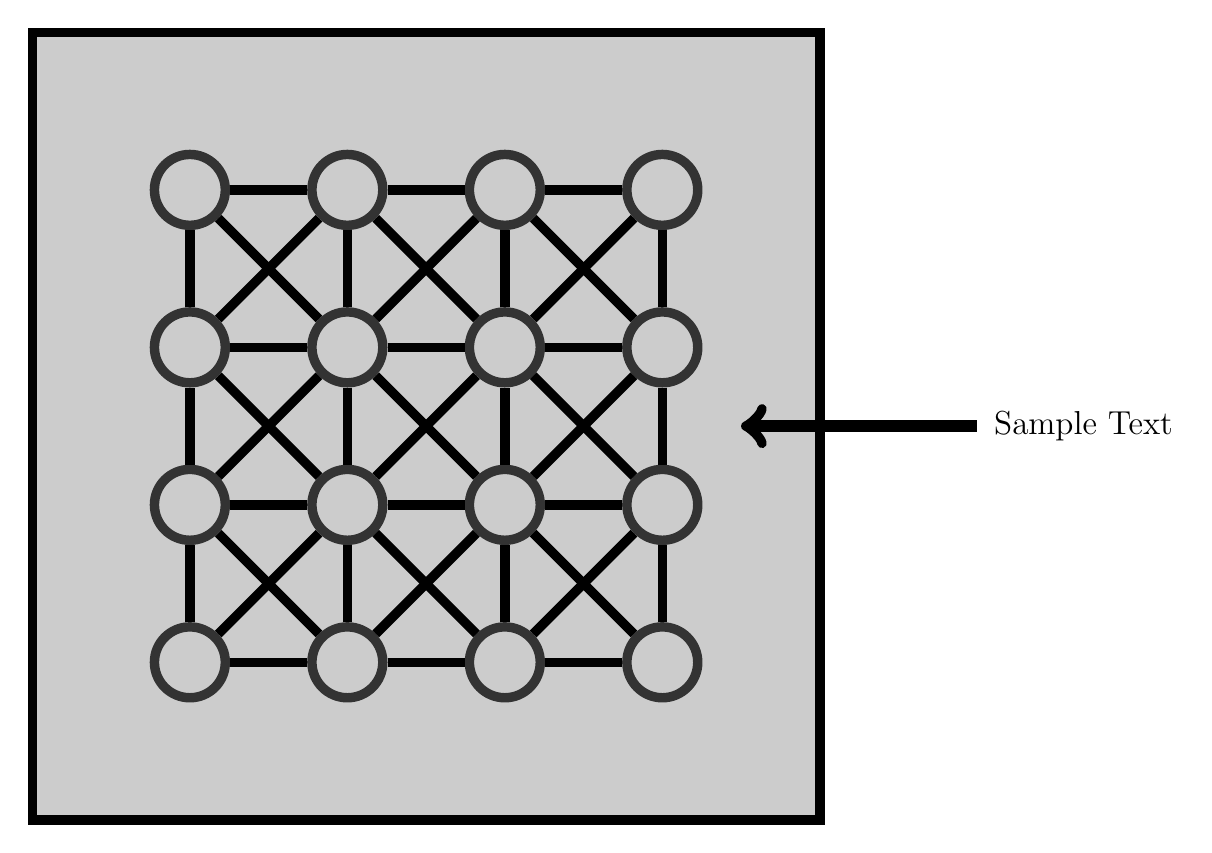
\begin{tikzpicture}


    \foreach \x in {-3,-1,...,3}{
        \foreach \y in {-3,-1,...,3}{
            \node (Image17_\x_\y) [draw=\squareColor,  thick, line width=\squareLineWidth, shape=circle, minimum width=\circleRadius,  anchor=center]  at (\x,\y) {};
        }
    }

    \filldraw[thin,gray,opacity=.4] (5,-5) rectangle (-5,5);


    %    \draw [-][draw=\squareColor,  thick, line width=\squareLineWidth] (Image17_1_3.east) -- (Image17_3_3.west);
    \draw [-][draw=\squareColor,  thick, line width=\squareLineWidth] (Image17_-3_-3.east) -- (Image17_-1_-3.west);
    \draw [-][draw=\squareColor,  thick, line width=\squareLineWidth] (Image17_-1_-3.east) -- (Image17_1_-3.west);
    \draw [-][draw=\squareColor,  thick, line width=\squareLineWidth] (Image17_1_-3.east) -- (Image17_3_-3.west);

    \draw [-][draw=\squareColor,  thick, line width=\squareLineWidth] (Image17_-3_-1.east) -- (Image17_-1_-1.west);
    \draw [-][draw=\squareColor,  thick, line width=\squareLineWidth] (Image17_-1_-1.east) -- (Image17_1_-1.west);
    \draw [-][draw=\squareColor,  thick, line width=\squareLineWidth] (Image17_1_-1.east) -- (Image17_3_-1.west);


    \draw [-][draw=\squareColor,  thick, line width=\squareLineWidth] (Image17_-3_1.east) -- (Image17_-1_1.west);
    \draw [-][draw=\squareColor,  thick, line width=\squareLineWidth] (Image17_-1_1.east) -- (Image17_1_1.west);
    \draw [-][draw=\squareColor,  thick, line width=\squareLineWidth] (Image17_1_1.east) -- (Image17_3_1.west);


    \draw [-][draw=\squareColor,  thick, line width=\squareLineWidth] (Image17_-3_3.east) -- (Image17_-1_3.west);
    \draw [-][draw=\squareColor,  thick, line width=\squareLineWidth] (Image17_-1_3.east) -- (Image17_1_3.west);
    \draw [-][draw=\squareColor,  thick, line width=\squareLineWidth] (Image17_1_3.east) -- (Image17_3_3.west);

%Part Two
    \draw [-][draw=\squareColor,  thick, line width=\squareLineWidth] (Image17_-3_-3.north) -- (Image17_-3_-1.south);
    \draw [-][draw=\squareColor,  thick, line width=\squareLineWidth] (Image17_-1_-3.north) -- (Image17_-1_-1.south);
    \draw [-][draw=\squareColor,  thick, line width=\squareLineWidth] (Image17_1_-3.north) -- (Image17_1_-1.south);
    \draw [-][draw=\squareColor,  thick, line width=\squareLineWidth] (Image17_3_-3.north) -- (Image17_3_-1.south);

    \draw [-][draw=\squareColor,  thick, line width=\squareLineWidth] (Image17_-3_-1.north) -- (Image17_-3_1.south);
    \draw [-][draw=\squareColor,  thick, line width=\squareLineWidth] (Image17_-1_-1.north) -- (Image17_-1_1.south);
    \draw [-][draw=\squareColor,  thick, line width=\squareLineWidth] (Image17_1_-1.north) -- (Image17_1_1.south);
    \draw [-][draw=\squareColor,  thick, line width=\squareLineWidth] (Image17_3_-1.north) -- (Image17_3_1.south);


    \draw [-][draw=\squareColor,  thick, line width=\squareLineWidth] (Image17_-3_1.north) -- (Image17_-3_3.south);
    \draw [-][draw=\squareColor,  thick, line width=\squareLineWidth] (Image17_-1_1.north) -- (Image17_-1_3.south);
    \draw [-][draw=\squareColor,  thick, line width=\squareLineWidth] (Image17_1_1.north) -- (Image17_1_3.south);
    \draw [-][draw=\squareColor,  thick, line width=\squareLineWidth] (Image17_3_1.north) -- (Image17_3_3.south);

%Part Three
    \draw [-][draw=\squareColor,  thick, line width=\squareLineWidth] (Image17_-3_3.south east) -- (Image17_-1_1.north west);
    \draw [-][draw=\squareColor,  thick, line width=\squareLineWidth] (Image17_-1_3.south east) -- (Image17_1_1.north west);
    \draw [-][draw=\squareColor,  thick, line width=\squareLineWidth] (Image17_1_3.south east) -- (Image17_3_1.north west);

    \draw [-][draw=\squareColor,  thick, line width=\squareLineWidth] (Image17_-3_1.south east) -- (Image17_-1_-1.north west);
    \draw [-][draw=\squareColor,  thick, line width=\squareLineWidth] (Image17_-1_1.south east) -- (Image17_1_-1.north west);
    \draw [-][draw=\squareColor,  thick, line width=\squareLineWidth] (Image17_1_1.south east) -- (Image17_3_-1.north west);

    \draw [-][draw=\squareColor,  thick, line width=\squareLineWidth] (Image17_-3_-1.south east) -- (Image17_-1_-3.north west);
    \draw [-][draw=\squareColor,  thick, line width=\squareLineWidth] (Image17_-1_-1.south east) -- (Image17_1_-3.north west);
    \draw [-][draw=\squareColor,  thick, line width=\squareLineWidth] (Image17_1_-1.south east) -- (Image17_3_-3.north west);

%Part Four
    \draw [-][draw=\squareColor,  thick, line width=\squareLineWidth] (Image17_-1_3.south west) -- (Image17_-3_1.north east);
    \draw [-][draw=\squareColor,  thick, line width=\squareLineWidth] (Image17_1_3.south west) -- (Image17_-1_1.north east);
    \draw [-][draw=\squareColor,  thick, line width=\squareLineWidth] (Image17_3_3.south west) -- (Image17_1_1.north east);

    \draw [-][draw=\squareColor,  thick, line width=\squareLineWidth] (Image17_-1_1.south west) -- (Image17_-3_-1.north east);
    \draw [-][draw=\squareColor,  thick, line width=\squareLineWidth] (Image17_1_1.south west) -- (Image17_-1_-1.north east);
    \draw [-][draw=\squareColor,  thick, line width=\squareLineWidth] (Image17_3_1.south west) -- (Image17_1_-1.north east);

    \draw [-][draw=\squareColor,  thick, line width=\squareLineWidth] (Image17_-1_-1.south west) -- (Image17_-3_-3.north east);
    \draw [-][draw=\squareColor,  thick, line width=\squareLineWidth] (Image17_1_-1.south west) -- (Image17_-1_-3.north east);
    \draw [-][draw=\squareColor,  thick, line width=\squareLineWidth] (Image17_3_-1.south west) -- (Image17_1_-3.north east);


%    end graph
    \node [draw=\squareColor,  thick, line width=\squareLineWidth, shape=rectangle, minimum width=\secondSquare, minimum height=\secondSquare, anchor=center] (Image18_Square_First) at (0,0) {};




    \draw [node font= \large, draw=\arrowColor,  thick, line width=\arrowLineWidth][<-]  (4,0) --(7,0) node[right] {\textArrow};


\end{tikzpicture}


\end{document}

